% Chapter 29: Why a Broken Cup Never Reassembles Itself (complete sample chapter)
\chapter{Why a Broken Cup Never Reassembles Itself}

\step{A Counterintuitive Opening}

Play a mental video: a hand releases a porcelain cup, which falls, strikes the floor, and breaks into a dozen pieces, splashing tea everywhere. Now play it \textbf{backward}: tea gathers from the floor, fragments rise and fit perfectly into a whole cup, and it jumps onto the table.

The reversed version looks absurdly fake. Any viewer recognizes reversal instantly, even without knowing physics.

Try more reversal tests. Blue ink spreads through clear water until it is uniformly pale blue; backward, the color gathers into one drop, obviously fake. Open perfume and its scent fills a room; backward, dispersed molecules turn together and queue into the bottle, obviously fake. Hot coffee cools on a table; backward, cool coffee gathers room heat and boils again, obviously fake. We have all used this instant-fake detector since childhood without asking how we recognize it.

Now a different video: two dust particles collide in water. One drifts toward the other, they strike and separate, each drifting away. Play it backward and nobody can tell: both versions look equally reasonable. More boldly, film two colliding air molecules and the reverse likewise looks flawless.

This is odd. Cups consist of molecules, and dust collisions are enlarged molecular collisions. If each microscopic collision is legal forward or backward, why do billions together acquire a distinct direction, allowing cups to break but not reassemble?

You may know that mechanics follows Newton's laws, none of which forbids fragments rejoining. Indeed, precisely reverse every molecule's velocity at the instant of fracture, and Newton's laws obediently restore the cup. Mechanics permits restoration. Yet it never happens, not once.

\begin{mainline}
Physics meets a strange crack: microscopic laws distinguish neither direction, while the macroscopic world takes only one. Something is missing between them. This chapter supplies \textbf{probability}.
\end{mainline}

\step{Make a Guess First}

Before continuing, write your guess. Which explanation is closest?

First: the floor eats the energy, leaving too little to restore the cup.

Second: an unknown force or law explicitly forbids broken objects becoming whole.

Third: restoration is allowed, but would require an extraordinary coincidence: billions of molecules all moving just right together, with probability effectively zero.

Do not choose hastily. Reassembly does not violate energy conservation. Breaking converts kinetic energy into molecular thermal motion and fracture energy; restoring it can turn those back into cup motion and material binding energy. The ledger can balance perfectly. Conservation cannot determine direction. What does?

This is no exaggerated puzzle. Nineteenth-century physics' best minds struggled with it. Kinetic theory explained gas properties through reversible collisions, yet could not explain why gases disperse rather than gather. Some even rejected atoms over this. First build intuition with your hands, then return to the dispute.

Remember which guess you chose. We will check it at the end. A wrong guess is no disgrace; forgetting your original thinking afterward is. Repeated recalibration builds physical intuition.

\step{Hands-on Experiment}

\begin{experiment}[Beans You Cannot Shake Back]
Find a transparent lidded box, such as a food container, and about twenty beans of each of two colors, perhaps red beans and mung beans.

First put every red bean on the left and every green bean on the right, with no partition, merely avoiding disturbance. Close the lid and look at the clear separation.

Second gently shake ten times. Open it: red and green are mixed.

Third, the crucial step: keep shaking a hundred or a thousand times, watching as you go. Can the beans separate back into red-left, green-right? Shake until your hands ache. Nobody in history has shaken mixed beans back into separation.
\end{experiment}

This almost laughably simple experiment poses \textbf{the same problem} as the broken cup. Beans remember no original arrangement, and each collision is legal in both directions. Yet mixing never reverses.

Make it more numerical. Put four coins heads up on a table, then close your eyes, shake and toss them, record their faces, and repeat dozens of times. How often all heads? How often two heads and two tails? A phone random-number program can substitute, producing four zeros or ones and counting all-zero versus two-zero-two-one outcomes. Results consistently favor two-and-two by about five or six times. Why that ratio? We will uncover the mechanism.

Record three more observations. Does more shaking mix beans more or less uniformly? With just one red and one green bean, is returning still difficult? Would two colors of fine sand change the conclusion? Write answers now; the concepts will address each.

\step{The Old Model Runs into Trouble}

Inventory the old models and where they stall.

Newtonian mechanics determines each bean's motion through collision forces and initial velocities. But its equations have a symmetry: replace time \(t\) with \(-t\) and they still hold. In Chapter 12's language, every legal process has a legal reverse. A vertically thrown ball reversed is a freely falling ball, both obeying one law. Mechanics cannot explain why we never see the cup's reverse.

Energy conservation cannot help either. We checked that restoration balances. Conservation governs total quantity, not direction, like an accountant checking totals without asking where money goes.

Perhaps friction heats things and the heat disperses, preventing reversal. Useful everyday language, but no ultimate answer. Heat is random molecular motion. Saying frictional heat makes things irreversible says mixed molecular motion cannot return, exactly the phenomenon requiring explanation. It smuggles the answer into the question.

Another dead end blames special initial conditions. Perhaps the universe happened to start extraordinarily specially, giving us a one-way street. That is substantially right, and the ending thought experiment revisits it, but merely shifts the question from cup to cosmic beginning. Even without asking about origins, beans and ink still need a quantitative account of direction.

\begin{mainline}
Compress the difficulty: \textbf{microscopic laws permit both directions, but the macroscopic world takes one; conservation governs quantity, not direction}. We need no new force, but a new counting method.
\end{mainline}

\step{Inventing New Concepts}

Now invent concepts ourselves. Return to four coins.

Number them 1, 2,3, 4. One macroscopic outcome is two heads and two tails. Its specific realizations are heads on 1 and 2, on 1 and 3, on 1 and 4, on 2 and 3, on 2 and 4, or on 3 and 4, with the other two tails: six arrangements. All heads has just one.

\begin{mainline}
Name the levels. A state described at a glance in macroscopic language, two heads/two tails, mixed beans, or broken cup, is a \textbf{macrostate}. Every member's precise arrangement, which coin faces up or each molecule's position and velocity, is a \textbf{microstate}. The number of microstates corresponding to one macrostate is \(\Omega\).
\end{mainline}

For four coins: all heads, \(\Omega=1\); three heads and one tail, \(\Omega=4\), choosing which coin is tails; two-and-two, \(\Omega=6\); one head and three tails, \(\Omega=4\); all tails, \(\Omega=1\). Their sum \(1+4+6+4+1=16\) equals \(2^4\): sixteen equally probable microstates. This explains the experimental five- or sixfold ratio: two-and-two has probability \(6/16\), exactly six times all-heads probability \(1/16\).

The key discovery: if microstates are equally likely, a macrostate's probability is proportional to \(\Omega\). \textbf{Coins do not prefer disorder; the two-and-two macrostate simply owns more microscopic realizations.} Red-left/green-right beans have very few arrangements, while mixed colors have mountains of them. Shaking moves randomly from a sparsely populated macrostate into a crowded one. Mixing needs no special reason, like walking into a hall; maintaining separation needs a miracle.

Replace beans with molecules and the picture stays, only the numbers change. Below, each box has an imaginary middle division and each dot is a molecule. All-left is low entropy, uniform distribution high entropy. The difference lies not in identical, unacquainted molecules, but in how many microscopic arrangements belong to each macrostate.

\begin{center}
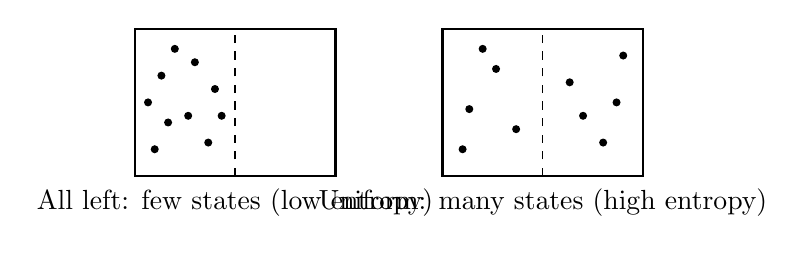
\begin{tikzpicture}[scale=0.85]
  % Left: all molecules in left half
  \draw[thick] (0,0) rectangle (3,2.2);
  \draw[dashed] (1.5,0) -- (1.5,2.2);
  \foreach \px/\py in {0.3/0.4, 0.8/0.9, 0.4/1.5, 1.1/0.5, 0.6/1.9, 1.2/1.3, 0.9/1.7, 0.2/1.1, 1.3/0.9, 0.5/0.8}
    \fill (\px,\py) circle (0.06);
  \node at (1.5,-0.4) {All left: few states (low entropy)};
  % Right: uniform distribution
  \begin{scope}[xshift=4.6cm]
  \draw[thick] (0,0) rectangle (3,2.2);
  \draw[dashed] (1.5,0) -- (1.5,2.2);
  \foreach \px/\py in {0.3/0.4, 0.8/1.6, 0.4/1.0, 1.1/0.7, 0.6/1.9, 1.9/1.4, 2.4/0.5, 2.7/1.8, 2.1/0.9, 2.6/1.1}
    \fill (\px,\py) circle (0.06);
  \node at (1.5,-0.4) {Uniform: many states (high entropy)};
  \end{scope}
\end{tikzpicture}
\end{center}

Delimit the hall analogy. \textbf{Where it works}: random walkers are likelier to occupy a larger room, as colliding molecules favor macrostates with more realizations. \textbf{Where it fails}: people have goals, tire, and avoid each other; molecules do not. Room size is fixed, whereas macrostate size, \(\Omega\), requires counting rather than visual measurement. Analogies get you through the door; counting makes the statement precise.

Boltzmann pursued this idea in the nineteenth century, assigning each macrostate a number measuring its microscopic multiplicity: \textbf{entropy}, \(S\). More microstates mean greater entropy. An isolated system spontaneously moves toward macrostates with more microstates, not because a force pushes it, but because random wandering almost certainly enters the largest room. The idea provoked fierce attacks on Boltzmann: many rejected invisible atoms and statistically derived direction. Today atomic images and direct fluctuation measurements have settled the dispute.

Immediately correct a common mistake: entropy as disorder. \textbf{Where it works}: tidy arrangements, all heads or separated colors, indeed have fewer realizations than mixed ones. \textbf{Where it fails} has three parts. Disorder is subjective, while \(\Omega\) is objectively countable: a tidy parent and untidy child may judge one room differently, but its multiplicity is one number. Some orderly structures actually help increase entropy: snow crystals are beautifully organized, yet crystallization releases heat, increasing the combined water-plus-surroundings multiplicity. Finally, disorder depends on macroscopic description: a deck disordered by factory standards may still be insufficiently shuffled by casino standards. Eyes can misjudge entropy. Here we speak only of multiplicity.

\step{The Model in One Sentence}

\begin{oneline}
A broken cup never reassembles not because laws forbid it, but because restoration has pitifully few microstates. Random evolution almost inevitably reaches macrostates with more realizations. Entropy measures that multiplicity.
\end{oneline}

Read it three ways. Not forbidden: direction grows from reversible laws plus counting, not a prohibition. Random evolution: the system has no goal; large numbers turn random wandering into an effectively definite direction. Measure: entropy has units, can be measured and calculated, and enters engine-efficiency formulas next chapter.

\step{The Mathematical Translator}

Translate more and fewer into numbers, and the contrast becomes more extreme than imagined.

First count coins. For \(N\) coins, exactly \(k\) heads has as many microstates as ways to select from \(N\) coins the \(k\) that show heads, written
\[
\Omega(N,k)=\binom{N}{k}=\frac{N!}{k!\,(N-k)!}.
\]
For four: \(\Omega(4,0)=1\), \(\Omega(4,2)=6\), \(\Omega(4,4)=1\), matching our count. Total microstates are
\[
\sum_{k=0}^{N}\binom{N}{k}=2^{N}.
\]

Check extremes: \(N=4\) gives \(2^4=16\), correctly. All heads, \(k=N\), gives \(\Omega=1\), one arrangement. For even \(N\), \(\Omega\) peaks at \(k=N/2\): exactly half heads has the most realizations.

The graph plots the four-coin macrostate, number of heads, against multiplicity \(\Omega\). A central bulge, low ends.

\begin{center}
\begin{tikzpicture}[scale=0.9]
  \draw[-{Stealth}] (0,0) -- (6.4,0) node[right] {Number of heads $k$};
  \draw[-{Stealth}] (0,0) -- (0,3.4) node[above] {$\Omega$};
  \fill[blue!40] (0.55,0) rectangle (1.05,0.25);
  \fill[blue!40] (1.95,0) rectangle (2.45,1.0);
  \fill[blue!40] (3.35,0) rectangle (3.85,1.5);
  \fill[blue!40] (4.75,0) rectangle (5.25,1.0);
  \fill[blue!40] (5.75,0) rectangle (6.25,0.25);
  \node at (0.8,0.5) {\small 1};
  \node at (2.2,1.25) {\small 4};
  \node at (3.6,1.75) {\small 6};
  \node at (5.0,1.25) {\small 4};
  \node at (6.0,0.5) {\small 1};
  \foreach \px/\kk in {0.8/0, 2.2/1, 3.6/2, 5.0/3, 6.0/4}
    \node at (\px,-0.35) {\small $\kk$};
\end{tikzpicture}
\end{center}

Watch the shape change with \(N\). At \(N=4\), the center is only several times the ends; at \(N=100\), exactly fifty heads has about \(10^{29}\) arrangements while all heads still has one. Greater departures from half make multiplicity fall exponentially. More coins narrow the distribution into a central needle. \textbf{Equal microscopic probabilities, amplified by combinatorics, become an almost ironclad macroscopic rule.}

For a hundred coins, all heads has probability \(1/2^{100}\), with \(2^{100}\) about \(1.27\times10^{30}\). Toss once a second since the Big Bang, about \(1.4\times10^{10}\) years or \(4.4\times10^{17}\) seconds ago, for roughly \(4\times10^{17}\) tosses, and the chance of seeing all heads is still only of order one in a hundred billion. Near half, say 45 to 55 heads, has probability over seventy percent. Tossing a hundred coins lets you watch a small arrow of time.

Feel how fiercely \(2^N\) grows. Ten coins give all heads about once in a thousand, attainable by luck; twenty, once in a million, rare in a lifetime; forty, once in a trillion, hopeless even with all humanity tossing. Each extra coin halves the extreme's chance, while molecular \(N\) is not dozens but of order \(10^{23}\). Irreversibility is no profound ban, merely the flattened landscape left by exponential growth.

\begin{mathbridge}
The real leap is taking logarithms. Large particle numbers make \(\Omega\) monsters such as \(10^{10^{23}}\), impossible to write directly. Boltzmann compressed these astronomical counts with a natural logarithm:
\[
S = k_{\mathrm{B}} \ln \Omega,
\]
where \(k_{\mathrm{B}}\approx1.38\times10^{-23}\ \mathrm{J/K}\), Boltzmann's constant, converts counts into units compatible with temperature and energy, joules per kelvin.

This formula adorns Boltzmann's tomb. Why this form? First, \(\ln\) turns multiplication into addition. Independent systems have \(\Omega=\Omega_1\Omega_2\), so \(S=S_1+S_2\): entropy adds like energy. Second, \(\ln\Omega\) increases monotonically with \(\Omega\), preserving multiplicity order. Third, coefficient \(k_{\mathrm{B}}\) makes counted entropy exactly match thermodynamic entropy defined from heat and temperature, as Chapter 30 shows.

Give the units intuition. Joules per kelvin means an energy-scale account associated with each degree of warming. Mixing a spoonful of hot water into cold gives total entropy change only of order \(10^{-3}\) joules per kelvin. Small-looking, but multiplied from a constant of order \(10^{-23}\)! Work backward and \(\Omega\) grows by roughly \(e\) to the power \(10^{20}\). One everyday spoonful multiplies microscopic possibilities unimaginably.

When is this useful? Approximately isolated systems with approximately equal-probability microstates. When is caution needed? A few-particle system or strong correlations can make fluctuations large enough to defeat almost certainty. The limits section returns to this.
\end{mathbridge}

Now a real-scale estimate. A mole of room air contains about \(6\times10^{23}\) molecules. What is the chance that all accidentally occupy the left half at one instant, leaving the right empty? Equal left/right chances give
\[
\frac{1}{2^{6\times10^{23}}}.
\]
How small? Its decimal representation begins with roughly \(1.8\times10^{23}\) zeros after the decimal point. At a millimeter per zero, the line would reach Earth--Sun and back hundreds of millions of times. Cup reassembly demands a comparable or greater coincidence, aligning not just positions but every molecular velocity. Never happens translates into this numerical degree of impossibility.

\begin{challenge}
Near-uniform molecular distribution has a precise shape, not merely high probability. If \(n\) molecules occupy the left half, \(n\) follows a binomial distribution, mean \(N/2\) and standard deviation \(\sqrt{N}/2\). Relative fluctuations are \(\sqrt{N}/N=1/\sqrt{N}\): larger \(N\), smaller relative fluctuations. One mole gives about \(1.3\times10^{-12}\), uniform to eleven decimal places. Macroscopic certainty emerges from underlying probability not because probability vanishes, but because large numbers suppress fluctuations.

Stirling's approximation, \(\ln N!\approx N\ln N-N\), gives exactly-half multiplicity for \(N\) coins as \(\binom{N}{N/2}\approx 2^{N}\sqrt{2/(\pi N)}\). Taking logs, \(\ln\Omega\approx N\ln 2\), hence entropy \(S\approx N k_{\mathrm{B}}\ln 2\), proportional to particle number. This extensivity starts thermodynamic equilibrium calculations.
\end{challenge}

\step{The Model's Limits}

Every model must state assumptions, domain, and misuses. This is no exception.

\textbf{First assumption: equally likely microstates.} Everything rests on equal probability of microscopic arrangements. Countless macroscopic isolated-system tests support this equal-probability principle, but it remains an assumption, not a theorem derived from Newton's laws. What guarantees it, and how much random colliding establishes equality, are deep statistical questions pursued in Chapter 31.

\textbf{Second assumption: a sufficiently large system.} Almost inevitable motion toward large \(\Omega\) gains its power from astronomical particle numbers. Shrink the system and the iron law softens into probability. Three coins give all heads with probability \(1/8\), hardly rare. Mixed beans fail to separate, but three coins readily return to all heads. The theory honestly predicts small-system exceptions to irreversibility.

A beautiful counterexample is pollen. Brown's 1827 observation of irregular motion in water was later explained by molecular impacts. For sufficiently small particles over sufficiently short times, fluctuating impacts can push them and do positive work. At micrometer and nanosecond scales, heat becomes work daily. Modern laboratories directly measure such fluctuations with micrometer beads and confirm statistical predictions precisely. The second law never says absolutely forbidden, but macroscopically almost inevitable. Treating it as an absolute ban on the same footing as energy conservation is a common misuse.

\textbf{Third assumption: isolation.} Open systems can flow uphill locally if they pay the surroundings enough. Refrigerators freeze orderly ice, greatly reducing local multiplicity, while rejecting more heat into the kitchen so the whole water-plus-air multiplicity increases. Life is grander: a fertilized egg becomes a precisely structured person, with striking local entropy reduction, but lifelong eating, breathing, and heat loss ensure total body-plus-surroundings entropy increases. \textbf{Life violates entropy increase is a false claim that secretly changes the system boundary.}

One abuse deserves its own warning. Popular entropy gets dragged into everything: untidy rooms, information-overloaded societies, divided teams. The issue is not whether conclusions are right, but that these claims do not refer to a countable \(\Omega\)-based physical quantity. Physical entropy has units, values, and equations; rhetorical entropy is a stylish synonym for mess. Ask simply how the claimed entropy is measured.

Yet entropy's counting idea genuinely traveled far beyond heat. Shannon sought a measure of uncertainty in a message and obtained the same mathematical form as Boltzmann entropy, since information also involves the logarithm of possibilities. Chapter 32 explores it. More remarkably, black-hole entropy is proportional to surface area, and a black hole has more microscopic realizations than anything else of equal volume: the universe's largest room is a black hole. From four coins to black holes, one counting key opens doors forty orders of magnitude apart.

\begin{mainline}
Operating instructions: for isolated, macroscopic, countable systems, entropy increase is nearly inevitable. Small systems permit fluctuation reversals; open systems permit local decrease at greater environmental cost. Outside these conditions, entropy talk is usually analogy, not physics.
\end{mainline}

\step{Explaining the Opening Phenomenon}

Return to the two videos.

A dust-particle collision is one event involving a few molecules. Reverse every participant's velocity and obtain another legal collision, with no fewer realizing microstates than forward motion. That is why you cannot distinguish directions; physics at this scale truly lacks an arrow.

Breaking a cup is different. The broken world, fragment positions and molecular thermal motions, has unimaginably many microstates. Fragments rejoining and jumping onto a table require ten quadrillion molecules simultaneously to occupy exquisitely precise positions and velocities. Relatively few microstates meet those requirements. The probability ratio again has enough zeros to reach the Sun. \textbf{Reversal is not illegal, just outrageously unlikely}, beyond even a universe's lifetime of waiting.

Ink, perfume, and coffee follow suit. Spread ink has vast multiplicity, one reassembled drop tiny multiplicity. The former happens daily, the latter never. Your instant-reversal detector is a probability detector trained by hundreds of millions of years of evolution.

This explains dispersed sound and warmed fragments during breaking. Mechanical energy becomes random molecular motion, the energy arrangement with greatest multiplicity. Energy scattered into heat resembles beans scattered into the box, never gathering again. This is Chapter 21's dissipation seen from two sides: energy flow there, multiplicity here. Energy remains, having moved into the largest room.

Answer the experiment's three observations. More shaking gives more uniform mixing because uniform states have the most realizations; random wandering only sinks deeper, never overshaking into separation. With two beans, returning is easy: arrangements have comparable chances, with both left at probability \(1/4\), illustrating the large-system boundary. Fine sand gives the same conclusion, since irreversibility counts realizations rather than selecting materials. Friction changes mixing speed, not direction.

Check the guesses. First, insufficient energy is wrong because restoration balances; conservation does not choose direction. Second, an explicit ban is wrong because Newton's laws welcome the reverse. Third is right: enormous probability disparities make time's arrow emerge macroscopically. Microscopic laws lack arrows; large numbers statistically produce one.

\step{Thought Experiments and Challenges}

\begin{thought}[Waiting for All Heads]
If the universe tosses coins forever, every outrageous coincidence eventually occurs. Poincaré's recurrence theorem says an isolated mechanical system, given enough time, returns arbitrarily close to its original microstate. Broken cups, dispersed heat, and mixed beans can in principle replay.

But consider the timescale. A room-sized system with about \(10^{26}\) particles has estimated recurrence time of order \(10^{10^{25}}\) years, an exponential tower. The universe is only \(1.4\times10^{10}\) years old. Treat that age as a second and recurrence still exceeds the time imagined by making every cosmic atom another universe and letting each live another lifetime. No conflict with experience: the theorem says return in principle; experience says you will never wait long enough. An exponential separates two true statements.
\end{thought}

\begin{thought}[The Demon's Door]
Imagine two well-mixed gases in a box, divided by a partition with a frictionless little door guarded by a demon. It lets fast left-arriving molecules go right and slow right-arriving ones go left. Eventually the right warms and the left cools, seemingly reducing entropy with no energy expense. Maxwell's demon troubled physicists for over a century. Where is the flaw? Hint: the demon must measure, remember, and erase memories. Erasing one bit itself releases heat and produces environmental entropy, balancing the account. Information is physical too. This stitches the chapter to information in Chapter 32 and the second law in Chapter 30.
\end{thought}

\begin{puzzles}
\item \textbf{The shuffle account.} A new deck is neatly ordered by suit and rank; thorough shuffling makes it look random. Has entropy increased? Use this chapter's language, explaining why tidy has one or few arrangements while untidy has astronomically many. Would an accidental return to factory order violate any law?

  \textit{Hint:} There are \(52!\approx 8\times10^{67}\) permutations. Tidy owns very few; untidy almost all. Returning to factory order has probability about \(10^{-68}\), breaking no law, merely a lottery you will never win. Whether deck arrangements count as entropy depends on the chosen macroscopic description, exposing the unreliability of disorder language.

\item \textbf{The dented table-tennis ball.} A dented ball placed in hot water restores its shape. What do its gas molecules do? Why do hot-water molecules not coordinate to avoid the dent and leave it depressed?

  \textit{Hint:} Hot water transfers energy to the internal gas, making molecular motion stronger with equally likely impacts in all directions. Avoiding the dent requires special velocity correlations among many molecules, occupying a negligible fraction of microstates. Uniform bombardment has greatest multiplicity.

\item \textbf{Two rooms, one ending.} In room A, spray perfume indoors. For room B, spray the same bottle outdoors in strong wind. Where does scent disperse faster? Do molecular laws differ, and what determines the rate?

  \textit{Hint:} The microscopic laws match. Macroscopic conditions differ: outdoor directed flow and larger space increase accessible realizations faster. Entropy direction agrees while rates may differ by orders of magnitude. This chapter supplies direction, not a timetable.

\item \textbf{The reverse refrigerator.} Someone claims refrigerators prove entropy can decrease and therefore refute the second law. Identify the two switched concepts, correcting each in one sentence.

  \textit{Hint:} First, system boundary: the refrigerated interior is not isolated, so include the heat-receiving surroundings. Second, entropy increase's nature: the law is statistical near-certainty, not an absolute ban. But a refrigerator is no challenge at all; it continually buys internal entropy reduction with a larger environmental increase.
\end{puzzles}

Beginning with an absurd reversed video, we found one key behind macroscopic irreversibility: counting, not force or prohibition. Microscopic multiplicities differ beyond everyday scales, crystallizing probability into direction. We also settled Chapter 21's unfinished dissipation account. Energy becoming less useful did not explain why that was a one-way street; now we know the street is entropy increase.

Next we fit this key into thermodynamics. If entropy selects direction, heat flowing hot to cold, limited engine efficiency, and unreachable absolute zero become versions of one answer. Chapter 31 develops counting into statistical physics, and Chapter 32 asks how information relates to entropy. This everyday broken cup has a long queue of subjects at its door.
